\documentclass[11pt, letterpaper]{article}
\usepackage[utf8]{inputenc}
\usepackage{graphicx}
\graphicspath{{images/}}
\usepackage{dingbat}
\usepackage{amsmath}
\usepackage{amssymb}
\title{ECE316 Lecture Note 1 by Prof. Xie - Spring 2017}
\author{Prof. Liang-Liang Xie}
\date{\today}

\begin{document}
\section{Combinational Analysis}
\subsection{Introduction}
\textbf{Example}: A communication system consists of 4 antennas

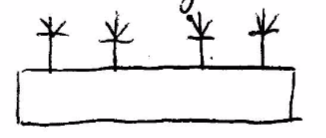
\includegraphics{1-1}

Assume that this system will be functional if no two consecutive antennas are defective. \newline \newline
\noindent
\underline{Q:} If there are exactly 2 antennas defective, what is the probability that the resulting system will be functional? \newline \newline
\noindent
\underline{Solution:}
\begin{center}
  \begin{tabular}{ c c c c c c }
    0 1 1 0 & 0 1 0 1 & 1 0 1 0 & 0 0 1 1 & 1 0 0 1 & 1 1 0 0 \\
    \checkmark & \checkmark & \checkmark & X & X & X
  \end{tabular}
\end{center}

If all the cases are equally likely, the probability is \( \frac{3}{6} \)=\( \frac{1}{2} \).

\subsection{The Basic Principle of Counting}
Suppose that two experiments are to be performed. If experiment 1 can result in any one of $m$ possible outcomes, and if for each outcome of experiment 1, there are $n$ possible outcomes of experiment 2, then together there are $m \times n$ possible outcomes of the two experiments.
\begin{center}
  \begin{tabular}{ c c c c }
    (1,1) & (1,2) & \dots & (1,n) \\
    (2,1) & (2,2) & \dots & (2,n) \\
    $\vdots$ & $\vdots$ & $\ddots$ & $\vdots$ \\
    (n,1) & (n,2) & \dots & (n,m)
  \end{tabular}
\end{center}
\textbf{Example}: A small community, 10 women, each has 3 children. If one women and one of her children are to be selected as mother and child of the year. How many possibilities? \newline
\noindent
\underline{Solution:} $10\times3 = 30$ \newline

\noindent\underline{Generalize:} \newline
Experiment 1 with $n_1$, possible outcomes, for each of them. There are $n_2$ outcomes of experiment 2, for each of them. There are $n_3$ possible outcomes of experiment 3\dots\dots then there are totally, \newline
\begin{equation*}
  n_1 \cdot n_2 \cdot n_3 \dots n_r
\end{equation*}
possible outfcomes of the r experiments.

\end{document}
